\documentclass{article}

\usepackage{amsmath}
\usepackage[margin=1in]{geometry}
\usepackage{natbib}
\usepackage{url}
\usepackage[pdftex]{graphicx}
\graphicspath{ {./results/} }

\title{Sharing Results with \LaTeX{} and \texttt{git}}
\author{Alexander L. Hayes \and You}
\date{}

\begin{document}

\maketitle

\section{Introduction}

\LaTeX{} is helpful for typesetting documents. Many conferences and
publication venues develop templates for typesetting papers at their
venue. A major feature is the mini language for typesetting
equations and formulas, like so:\footnote{This mini language now
shows up in many places where people typeset formulas, from Wikipedia to the
Mathematics StackExchange. See also: KaTeX \url{https://katex.org/}
or MathJax \url{https://www.mathjax.org/}.}

$$\mathrm{P}(y | x) = \frac{\mathrm{P}(x | y)\mathrm{P}(y)}{\mathrm{P}(x)}$$

$$\theta = (\mathbf{X}^{\top}\mathbf{X})^{-1} \mathbf{X}^{\top} \mathbf{y}$$

\section{A Concrete Problem}

You're reading Twitter and stumble across a tweet discussing an unusual pricing
procedure at a restaurant that serves chicken wings. You know data science,
so you dive into the data immediately.

\section{Finished Problem}

There it is 

\begin{figure}[h]
    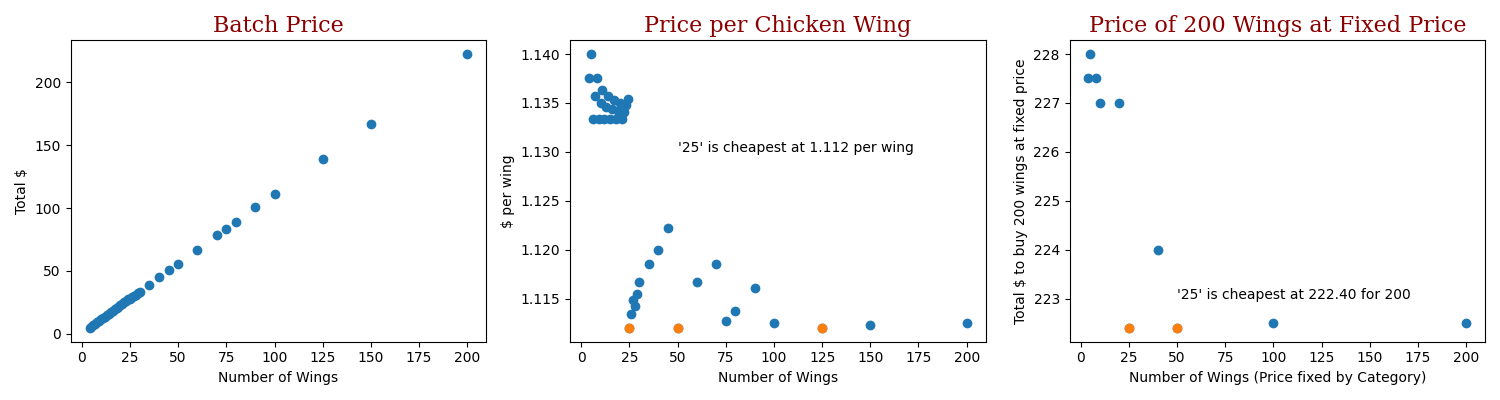
\includegraphics[width=\textwidth]{chicken_wing_plots.png}
    \caption{This figure was automatically generated with the
    \texttt{plot\_data.py} script in the \texttt{results} directory.
    (\textbf{Left}): What is the relationship between the (Number of
    chicken wings) and the (Total Price)---this appears to be
    approximately linear, with more wings costing more than fewer wings.
    (\textbf{Middle}): The price per chicken wing, computed by dividing
    the number of wings by the price, revealing that buying 25, 50, or
    125 wings is the cheapest option.
    (\textbf{Right}): What is the cheapest way to buy exactly 200 wings?
    This only shows cases that are evenly divisible,
    otherwise we'd have an instance of a knapsack problem.~\citep{wiki:Knapsack_problem}}
\end{figure}

\bibliographystyle{plainnat}
\bibliography{main}

\end{document}
